%% abtex2-modelo-relatorio-tecnico.tex, v-1.9.7 laurocesar
%% Copyright 2012-2018 by abnTeX2 group at http://www.abntex.net.br/ 
%%
%% This work may be distributed and/or modified under the
%% conditions of the LaTeX Project Public License, either version 1.3
%% of this license or (at your option) any later version.
%% The latest version of this license is in
%%   http://www.latex-project.org/lppl.txt
%% and version 1.3 or later is part of all distributions of LaTeX
%% version 2005/12/01 or later.
%%
%% This work has the LPPL maintenance status `maintained'.
%% 
%% The Current Maintainer of this work is the abnTeX2 team, led
%% by Lauro César Araujo. Further information are available on 
%% http://www.abntex.net.br/
%%
%% This work consists of the files abntex2-modelo-relatorio-tecnico.tex,
%% abntex2-modelo-include-comandos and abntex2-modelo-references.bib
%%

% ------------------------------------------------------------------------
% ------------------------------------------------------------------------
% abnTeX2: Modelo de Relatório Técnico/Acadêmico em conformidade com 
% ABNT NBR 10719:2015 Informação e documentação - Relatório técnico e/ou
% científico - Apresentação
% ------------------------------------------------------------------------ 
% ------------------------------------------------------------------------

\documentclass[
	% -- opções da classe memoir --
	12pt,				% tamanho da fonte
	openright,			% capítulos começam em pág ímpar (insere página vazia caso preciso)
	oneside,			% para impressão em recto e verso. Oposto a oneside
	a4paper,			% tamanho do papel. 
	% -- opções da classe abntex2 --
	%chapter=TITLE,		% títulos de capítulos convertidos em letras maiúsculas
	%section=TITLE,		% títulos de seções convertidos em letras maiúsculas
	%subsection=TITLE,	% títulos de subseções convertidos em letras maiúsculas
	%subsubsection=TITLE,% títulos de subsubseções convertidos em letras maiúsculas
	% -- opções do pacote babel --
	english,			% idioma adicional para hifenização
	french,				% idioma adicional para hifenização
	spanish,			% idioma adicional para hifenização
	brazil,				% o último idioma é o principal do documento
	]{abntex2}


% ---
% PACOTES
% ---

% ---
% Pacotes fundamentais 
% ---
\usepackage{lmodern}			% Usa a fonte Latin Modern
\usepackage[T1]{fontenc}		% Selecao de codigos de fonte.
\usepackage[utf8]{inputenc}		% Codificacao do documento (conversão automática dos acentos)
\usepackage{indentfirst}		% Indenta o primeiro parágrafo de cada seção.
\usepackage{color}				% Controle das cores
\usepackage{graphicx}			% Inclusão de gráficos
\usepackage{microtype} 			% para melhorias de justificação
\usepackage{pdfpages}
\usepackage{lscape}
\usepackage{tikz}
\usepackage{geometry}
\usepackage{pdflscape}
\usetikzlibrary{shapes.gates.logic.US,trees,positioning,arrows}
\newcommand{\under}{\underline{ }}
\usetikzlibrary{arrows,automata}
\usetikzlibrary{positioning}
\usepackage{tikz-uml}
% ---
% Pacotes adicionais, usados no anexo do modelo de folha de identificação
% ---
\usepackage{multicol}
\usepackage{multirow}
% ---
	
% ---
% Pacotes adicionais, usados apenas no âmbito do Modelo Canônico do abnteX2
% ---
\usepackage{lipsum}				% para geração de dummy text
% ---

% ---
% Pacotes de citações
% ---
\usepackage[brazilian,hyperpageref]{backref}	 % Paginas com as citações na bibl
\usepackage[alf]{abntex2cite}	% Citações padrão ABNT

% --- 
% CONFIGURAÇÕES DE PACOTES
% --- 

% ---
% Configurações do pacote backref
% Usado sem a opção hyperpageref de backref
\renewcommand{\backrefpagesname}{Citado na(s) página(s):~}
% Texto padrão antes do número das páginas
\renewcommand{\backref}{}
% Define os textos da citação
\renewcommand*{\backrefalt}[4]{
	\ifcase #1 %
		Nenhuma citação no texto.%
	\or
		Citado na página #2.%
	\else
		Citado #1 vezes nas páginas #2.%
	\fi}%
% ---

% ---
% Informações de dados para CAPA e FOLHA DE ROSTO
% ---
\titulo{Proposta de modelagem de banco de dados NoSQL}
\autor{Vanessa Martinez Tonini}
\local{São Paulo}
\data{2019}
\instituicao{%
  Universidade de São Paulo -- USP
  \par
  Instituto de Matemática e Estatística
  \par
  Programa de Pós-Graduação}
\tipotrabalho{Exercício}
% O preambulo deve conter o tipo do trabalho, o objetivo, 
% o nome da instituição e a área de concentração 
\preambulo{Proposta de modelagem para uma banco de dados NoSQL baseado no modelo de dados de agregados.}
% ---
 
% ---
% Configurações de aparência do PDF final

% alterando o aspecto da cor azul
\definecolor{blue}{RGB}{41,5,195}

% informações do PDF
\makeatletter
\hypersetup{
     	%pagebackref=true,
		pdftitle={\@title}, 
		pdfauthor={\@author},
    	pdfsubject={\imprimirpreambulo},
	    pdfcreator={LaTeX with abnTeX2},
		pdfkeywords={abnt}{latex}{abntex}{abntex2}{relatório técnico}, 
		colorlinks=true,       		% false: boxed links; true: colored links
    	linkcolor=blue,          	% color of internal links
    	citecolor=blue,        		% color of links to bibliography
    	filecolor=magenta,      		% color of file links
		urlcolor=blue,
		bookmarksdepth=4
}
\makeatother
% --- 

% --- 
% Espaçamentos entre linhas e parágrafos 
% --- 

% O tamanho do parágrafo é dado por:
\setlength{\parindent}{1.3cm}

% Controle do espaçamento entre um parágrafo e outro:
\setlength{\parskip}{0.2cm}  % tente também \onelineskip

% ---
% compila o indice
% ---
\makeindex
% ---

% ----
% Início do documento
% ----
\begin{document}


% Seleciona o idioma do documento (conforme pacotes do babel)
%\selectlanguage{english}
\selectlanguage{brazil}

% Retira espaço extra obsoleto entre as frases.
\frenchspacing 

% ----------------------------------------------------------
% ELEMENTOS PRÉ-TEXTUAIS
% ----------------------------------------------------------
% \pretextual

% ---
% Capa
% ---
\imprimircapa
% ---

% ---
% Folha de rosto
% (o * indica que haverá a ficha bibliográfica)
% ---
\imprimirfolhaderosto*
% ---


% ---
% RESUMO
% ---

% resumo na língua vernácula (obrigatório)
% \setlength{\absparsep}{18pt} % ajusta o espaçamento dos parágrafos do resumo
% \begin{resumo}
%  Segundo a \citeonline[3.1-3.2]{NBR6028:2003}, o resumo deve ressaltar o
%  objetivo, o método, os resultados e as conclusões do documento. A ordem e a extensão
%  destes itens dependem do tipo de resumo (informativo ou indicativo) e do
%  tratamento que cada item recebe no documento original. O resumo deve ser
%  precedido da referência do documento, com exceção do resumo inserido no
%  próprio documento. (\ldots) As palavras-chave devem figurar logo abaixo do
%  resumo, antecedidas da expressão Palavras-chave:, separadas entre si por
%  ponto e finalizadas também por ponto.

%  \noindent
%  \textbf{Palavras-chaves}: latex. abntex. editoração de texto.
% \end{resumo}
% ---


% ---
% inserir o sumario
% ---
\pdfbookmark[0]{\contentsname}{toc}
\tableofcontents*
\cleardoublepage
% ---

% ----------------------------------------------------------
% ELEMENTOS TEXTUAIS
% ----------------------------------------------------------
% \textual

% ----------------------------------------------------------
% Introdução (exemplo de capítulo sem numeração, mas presente no Sumário)
% ----------------------------------------------------------
% \chapter*[Introdução]{Introdução}
% \addcontentsline{toc}{chapter}{Introdução}

% Este documento e seu código-fonte são exemplos de referência de uso da classe
% \textsf{abntex2} e do pacote \textsf{abntex2cite}. O documento 
% exemplifica a elaboração de relatórios técnicos e/ou científicos produzidos
% conforme a ABNT NBR 10719:2015 \emph{Informação e documentação - Relatório
% técnico e/ou científico - Apresentação}.

% A expressão ``Modelo canônico'' é utilizada para indicar que \abnTeX\ não é
% modelo específico de nenhuma universidade ou instituição, mas que implementa tão
% somente os requisitos das normas da ABNT. Uma lista completa das normas
% observadas pelo \abnTeX\ é apresentada em \citeonline{abntex2classe}.

% Sinta-se convidado a participar do projeto \abnTeX! Acesse o site do projeto em
% \url{http://www.abntex.net.br/}. Também fique livre para conhecer,
% estudar, alterar e redistribuir o trabalho do \abnTeX, desde que os arquivos
% modificados tenham seus nomes alterados e que os créditos sejam dados aos
% autores originais, nos termos da ``The \LaTeX\ Project Public
% License''\footnote{\url{http://www.latex-project.org/lppl.txt}}.

% Encorajamos que sejam realizadas customizações específicas deste exemplo para
% universidades e outras instituições --- como capas, folhas de rosto, etc.
% Porém, recomendamos que ao invés de se alterar diretamente os arquivos do
% \abnTeX, distribua-se arquivos com as respectivas customizações.
% Isso permite que futuras versões do \abnTeX~não se tornem automaticamente
% incompatíveis com as customizações promovidas. Consulte
% \citeonline{abntex2-wiki-como-customizar} para mais informações.

% Este documento deve ser utilizado como complemento dos manuais do \abnTeX\ 
% \cite{abntex2classe,abntex2cite,abntex2cite-alf} e da classe \textsf{memoir}
% \cite{memoir}. 

% Equipe \abnTeX 

% Lauro César Araujo


% ----------------------------------------------------------
% PARTE - preparação da pesquisa
% ----------------------------------------------------------

% ---
\chapter{Motivação}
% ---
% ---

\section{Contextualização}

Alguns ex-alunos do IME-USP fundaram uma startup para o desenvolvimento de sistemas de recomendação na área de entretenimento e cultura e, como um passo inicial para a sua inserção nesse mercado, decidiram criar um site de referência sobre a produção cinematográfica brasileira. Esse site funcionará como uma interface de acesso amigável para um banco de dados (BD) com informações sobre filmes, séries e videoclipes musicais produzidos no país.

\section{Da tarefa}
Com base no contexto, esta atividade se dá em projetar um ou mais esquemas de BD NoSQL para armazenar os dados de forma a atender eficientemente os requisitos descritos a seguir. 

% ---
\chapter{Requisitos de dados}
% ---
% ---
Para cada produção catalogada nesse BD, deseja-se manter informações básicas de caracterização, tais como: título, ano da produção, duração, classificação etária, categorias (drama, comédia, romance, musical, etc.), países envolvidos na produção, empresa produtora, seus diretores e atores, bem como os nomes dos papéis desempenhados por cada ator.

\begin{itemize}
  \item As produções podem ter outros dados mais específicos, em função do seu tipo. Por exemplo, para um videoclipe, é preciso também manter os dados sobre a música divulgada, o cantor (ou cantores, no caso de um grupo musical) e o gênero (rock, samba, funk, etc.). Para os filmes, deseja-se manter informações sobre a bilheteria (total de espectadores que assistiram o filme) e faturamento. Um filme pode ser a sequência de outro filme; essa informação precisa estar no BD.
  \item As séries são divididas em temporadas que, por sua vez, são divididas em episódios. Uma série tem um nome e seus atores e diretores principais (que podem mudar com o passar do tempo). Além disso, cada episódio é um vídeo individual, que pode ter atores e diretores diferentes dos de um outro episódio na mesma série.
  \item Sobre os artistas (atores, músicos, diretores, etc.), o BD deve manter informações tais como o nome, a data e local de nascimento, um texto (curto) de biografia e a data de morte (caso o artista já tenha falecido). Um artista pode ser “multifacetado”; por exemplo, a Jeniffer Lopez é cantora e atriz.
  \item Junto com as informações sobre uma produção, o site deverá exibir uma nota média de avaliação e algumas opiniões sobre o filme, que serão obtidas dos usuários cadastrados no site. Um usuário que esteja “logado” ao site poderá tanto avaliar uma produção quanto a atuação de um dado ator na produção, por meio da atribuição de uma nota de 0 a 5 e da escrita de um comentário.
  \item Os usuários poderão também dar notas (entre 0 e 5) aos comentários feitos por outros usuários. E os usuários que possuam uma boa avaliação de seus comentários ganham um tipo de acesso privilegiado ao site, que permitirá que eles cadastrem dados de novas produções e que também escrevam reviews que serão exibidos com destaque no site, junto aos dados das produções correspondentes.
\end{itemize}

% ---
\chapter{Requisitos de funcionais}
% ---
% ---
\begin{enumerate}
  \item Recuperar dados dos vídeos dirigidos por um dado diretor;
	\item Recuperar dados dos videoclipes de um dado grupo musical;
	\item Obter os nomes de atores que já atuaram como diretor (ou vice-versa);
	\item Obter dados dos filmes que são comédias musicais;
	\item Obter todas as sequências (diretas e indiretas) de um dado filme;
	\item Obter os nomes de atores que atuaram em uma dada série;
	\item Obter a nota média de uma produção ou de uma atuação;
	\item Obter a lista de produções mais bem avaliadas na última semana;
	\item Obter os identificadores dos usuários que fizeram os comentários mais bem avaliados no último mês.
\end{enumerate}

% ---
\chapter{Pesquisa}
% ---
% ---

\section{Escolha do tipo do banco de dados}

O tipo de banco de dados usa do para fazer a proposta da modelagem será o de documentos. Esta escolha é baseada na popularidade do uso pelo mercado e sucesso do mesmo, com implementações hoje já maduras e estabilizadas, como o MongoDB.

\section{Padrões de modelagem NoSQL}
Pelo fato de um banco de dados de documentos ter a possibilidade de atuar sem um Schema, não significa que ele não poderá ter um Schema. E muito pelo contrário, os autores do MongoDB recomendam fortemente o uso de um Schema para modelar um banco de dados NoSQL, assim diminuindo os impactos da possível inconsistência de dados.

Com isto, estes mesmos os autores, disponibilizaram uma série de padrões de modelagem do banco de dados no blog do MongoDB, criadas à partir do conhecimento adquirido na consultoria à clientes, representados na figura 1.

\begin{tikzpicture}
	\pgftext{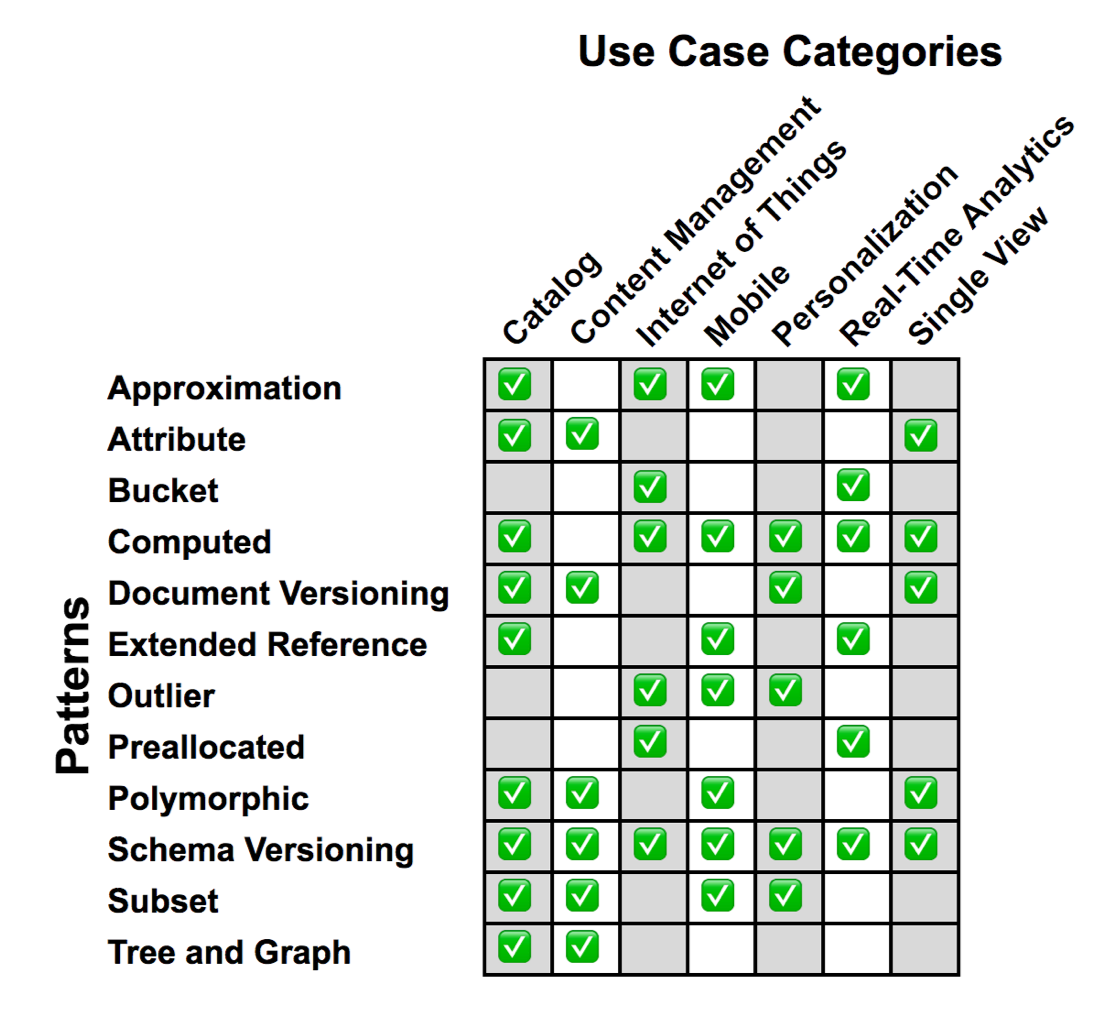
\includegraphics[width=300pt]{./imagens/patternsmatrix.png}}
\end{tikzpicture}

Os padrões propostos não são excludentes, ou seja, é possível implementar mais de um padrão em uma solução. Portanto escolhi 4 destes padrões que contribuem a necessidade de uso dos dados com base nos requisitos funcionais. São eles:

\begin{enumerate}
  \item \textbf{Attribute Pattern} (padrão de atributos): diminuí o indexamento de atributos parecidos, transportando-os para uma estrutura de lista;
  \item \textbf{Polymorphic Pattern} (padrão polimórfico): o mesmo documento tem diferentes formatos porém compartilha de muitos atributos em comum. Então agrupa-se os documentos com base nas "queries" que necessitamos fazer. Com isto, ameniza a necessidade de fazer "joins" complexos;
  \item \textbf{Outlier Pattern} (padrão fora da curva): usado quando o fator "popularidade" acontece, e um documento tem seu tamanho aumentado considerávelmente (por exemplo 16Mb). Para isto, cria-se um atributo "flag" que sinalizará este fator em determinado documento e transportará os dados excedentes para um ou mais documentos (estes chamados de "overflow documents"), deixando apenas um número limitado no documento principal. Este padrão evita mudar todo um Schema por causa de um fato isolado;
  \item \textbf{The Computed Pattern} (o padrão computado): quando temos dados que precisam ser computados repetitivamente, ou a partir de outros dados. Também serve para quando há mais leitura do que escrito de dados. E bom para quando precisa ser montada listas como "100 melhores ...";
  \item \textbf{Subset Pattern} (padrão subconjunto): Quando o alocamento de memória RAM é alto devido ao tamanho dos documentos. Resulta em dados sendo removidos da memória RAM criando um subconjunto de dados menos usados (similar ao Outlier Pattern).
\end{enumerate}

% ---
\chapter{Escolha da abordagem}
% ---
% ---
As chaves artificiais são geradas automaticamante pelo sistema de banco de dados no momento em que um dado do tipo object é feito. Estes objetos recebem uma chave com o nome "{\under}id" onde esta já vem as regras de unicidade, e geralmente são uma hash.

% ---
% Finaliza a parte no bookmark do PDF
% para que se inicie o bookmark na raiz
% e adiciona espaço de parte no Sumário
% ---
\phantompart 
\chapter{Apresentação do modelo}
O modelo

\newgeometry{margin=1cm}
\begin{landscape}
\thispagestyle{empty} %% Remove header and footer.
\tikzumlset{font=\tiny\ttfamily}
\begin{center}
	\textbf{Diagrama de entidades}
\end{center}
	\begin{tikzpicture}

	% entidades
		% pacote producao
			\umlclass[x=0,y=1]{Producao}{  
				titulo: string \\ 
				resumo: string \\ 
				descricao: string \\
				cadastradoPor: string \\
				genero: string \\
				videoTrailer: string \\
				ano: numeric \\
				duracao: numeric \\
				classificacaoEtaria: numeric \\
				mediaAvaliacao: numeric \\
				popular: boolean \\
				paisesProdutoresId: string[] \\
				produtorasId: string[] \\
				estreandoArtistaId: string[] \\
				diretoresId: string[]\\
				tipo: object<Filme | Serie> \\
				avaliacaoDosUsuarios: object[]
			}{}
	
			\umlclass[x=6,y=0]{Filme}{  
				bilheteria: numeric \\ 
				faturamento: numeric \\ 
				sequencia: object \\ 
				personagens: object[] \\
				avaliacaoArtista: object[] \\
			}{}

			\umlclass[x=6,y=-5]{Serie}{  
				qtdTemporadas: numeric \\
				personagens: object[] \\
				episodios: object[]
			}{}
	
			\umlclass[x=6,y=4]{Sequencia}{  
				ordem: numeric \\ 
				antecessorId: string \\ 
				sucessorId: string \\ 
			}{}
	
			\umlclass[x=11,y=0]{Personagens}{  
				nome: string \\ 
				atuadoPorId: string \\ 
			}{}
	
			\umlclass[x=14,y=4]{AvaliacaoArtista}{  
				artistaId: string \\ 
				notaMedia: numeric \\ 
				avaliacao: object \\ 
			}{}
	
			\umlclass[x=18,y=4]{Avaliacao}{  
				usuarioId: string \\ 
				nota: numeric \\ 
			}{}
	
			\umlclass[x=13,y=-5.5]{Episodio}{  
				numero: numeric \\
				temporada: numeric \\
				atoresConvidadosId: string[] \\
				diretoresConvidadosId: string[] \\
				personagensConvidados: object[] \\
				avaliacaoArtista: object[] \\
			}{}
	
			\umlclass[x=0,y=-6]{AvaliacaoDosUsuarios}{  
				data: string \\
				usuarioId: string \\
				producaoId: string \\
				nota: numeric \\
				comentario: object
			}{}
	
			\umlclass[x=0,y=-10]{Comentario}{  
				conteudo: string \\
				nota: numeric \\
				avaliacoesComentarioId: string[]
			}{}

		\umlclass[x=18,y=-1]{Artista}{  
			nome: string \\
			miniBiografia: string \\
			dataDeObito: string \\
			dataDeNascimento: string \\
			localDeNascimento: string \\
			atuouEmId: string[] \\
			atuacaoTipo: object \\
		}{}

		\umlclass[x=23,y=-1]{AtuacaoTipo}{  
			musical: boolean \\
			cinema: boolean \\
			direcao: boolean \\
			grupoMusical: boolean \\
		}{} 

		\umlclass[x=6,y=-10]{Usuario}{  
			nome: string \\
			sobrenome: string \\
			nomeDeUsuario: string \\
			email: string \\
			senha: string \\
			cidade: string \\
			notaPorAvaliacoes: numeric \\
			usuarioPrivilegiado: boolean \\ 
			avaliacoesFeitasId: string[] \\
		}{}

		\umlclass[x=11,y=-10]{Produtora}{  
			nome: string \\
			pais: string \\
		}{}

		\umlclass[x=16,y=-10]{Generos}{  
		}{
			nome: string \\ 
			producoesId: string[] \\ 
			musical: boolean \\ 
			visual: boolean \\ 
		}

		\umlclass[x=22,y=-10]{Resenhas}{  
		}{
			titulo: string \\
			data: string \\
			autorId: string \\
			resumo: string \\
			conteudo: string \\
		}

		\umlunicompo[geometry=-|-]{Producao}{Filme} 
		\umlunicompo[geometry=-|-]{Producao}{Serie}
		\umlunicompo[mult1=1,mult2=*]{Producao}{AvaliacaoDosUsuarios}
		
		\umlassoc{AvaliacaoDosUsuarios}{Comentario}

		\umlassoc{Filme}{Sequencia}
		\umlassoc{Filme}{Personagens}
		\umlassoc{Filme}{AvaliacaoArtista}
		\umlassoc{AvaliacaoArtista}{Avaliacao}
		
		\umlassoc{Serie}{Personagens}
		\umlassoc{Serie}{Episodio}
		\umlassoc{Episodio}{Personagens}
		\umlassoc{Episodio}{AvaliacaoArtista}

		\umlassoc{Artista}{AtuacaoTipo}


	\end{tikzpicture}
\end{landscape}
\restoregeometry


% ---
% Conclusão
% ---
\chapter{Conclusão}
% --- 


% ----------------------------------------------------------
% ELEMENTOS PÓS-TEXTUAIS
% ----------------------------------------------------------
\postextual


% ----------------------------------------------------------
% Referências bibliográficas
% ----------------------------------------------------------


\bibliography{modelagem-nosql}




\end{document}
